\section{Algorithms}
\label{sec:algos}
\paragraph{}In this section we aim to describe in detail, and independently, the various reconstruction algorithms developed in order to perform shower reconstruction. These algorithms are elements in a reconstruction chain, which is flexible. Algorithms can be swapped and switched according to a user's specific needs. There may be different algorithms trying to reconstruct the same quantities, better suited to work in different scenarios. We first spend time describing each algorithm individually, and then provide those which are the algorithm chains currently in use.
\paragraph{}Each algorithm is referenced by the name given to the C++ class used for that algorithm.

\subsection{StartPoint3DModule}
\paragraph{}This algorithm reconstructs a 3D point which should represent the 1st charge deposition point of the shower in the TPC (i.e. the shower vertex). The input used are the 2D start points reconstructed for all clusters associated with the shower on the various planes. As a first step, the two clusters spanning the longest wire-range are selected. Information from the two 2D start points for these clusters is then combined to obtain a 3D start point. The x-position is reconstructed by averaging the time-coordinate position of the two 2D start-points. The (Y,Z) coordinate is reconstructed by finding the intersection point of the two wires (on distinct planes) on which the 2D start-points are found. {\color{red} Currently in the case in which two wires don't intersect, or don't intersect in the TPC, which are both possible outcomes, nothing is done to exclude the reconstructed 3D start-point ad a valid start-point.}

\subsection{Angle3DFormula}
\paragraph{}This module uses the 2D reconstructed direction from each cluster, and combines multiple 2D directions to obtain a single 3D direction for the shower. Two or more 2D angles from a subset of the 3 views can be combined to form a 3D angle by using the formulas shown in Fig.~\ref{fig:Angle3DFormula}~\cite{bib:showerreco3DDir}.
\begin{figure}[H]
\centering
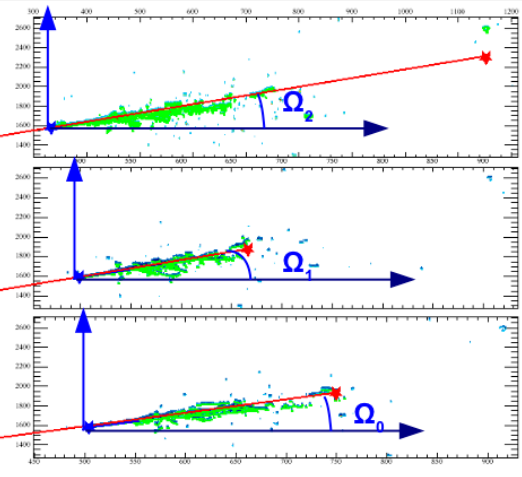
\includegraphics[width=0.35\textwidth]{figures/Angle3DFormula_00.png}
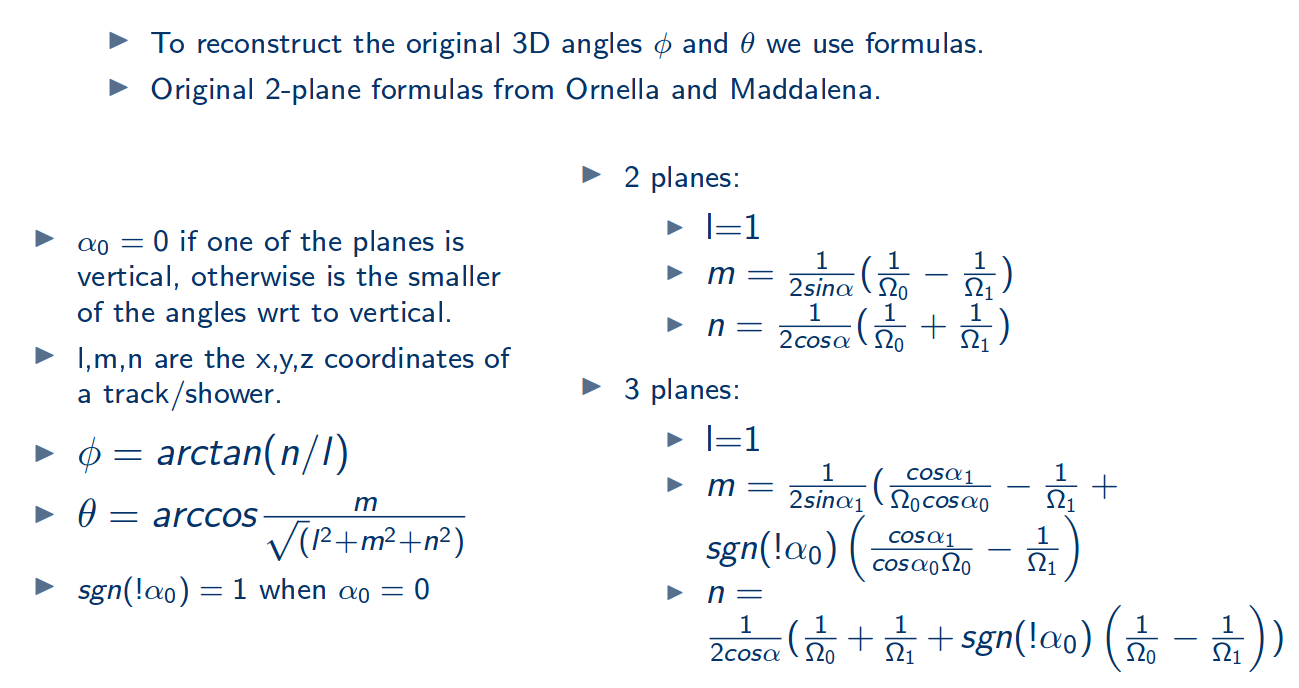
\includegraphics[width=0.55\textwidth]{figures/Angle3DFormula_01.png}
\caption{Left: schematic showing the 2D angles measured on all three planes for a given shower-like cluster. Right: formulae which are used by the Angle3DFormula to go form the 2D angles to a 3D direction.}
\label{fig:Angle3DFormula}
\end{figure}

\subsection{Angle3DFrmVtx}
\paragraph{}This module computes a 3D direction given two 3D points, representing the 3D vertex where the shower was produced, and the 3D start point of the shower (where it first deposits energy). This algorithm requires that a single 3D vertex has been loaded in the \texttt{ProtoShower} object. The purpose of this algorithm is to reconstruct a good 3D direction provided a vertex (tipically the neutrino vertex) has been reconstructed. The algorithm is intended mostly to be used for a photon sample.
\paragraph{}Given the reconstructed 3D start point of a shower, and the reconstructed vertex of origin for the electron or photon which initiates the shower, the 3D direction is given by:
\begin{equation}
{\rm 3Ddir} = \frac{ {\rm 3DStart} - {\rm 3Dvtx} }{ |{\rm 3DStart} - {\rm 3Dvtx}| }
\end{equation}

\subsection{dQdxModule}
\paragraph{}This algorithm aims to calculate the dQ/dx for the first few centimeters of energy deposition of the shower in each plane. The algorithm takes as input:
\begin{itemize}
\item Shower's reconstructed 3D direction.
\item Hits associated to the shower in a given plane.
\item 2D start point of each cluster.
\item 2D showering point of each cluster.
\item 2D opening angle of each cluster.
\end{itemize}
For each cluster, the \texttt{ClusterRecoUtil} toolkit provides a reconstructed start point and showering point. These are meant to represent the point at which the shower begins to deposit charge in the detector (the shower's vertex on the plane) and the point at which the shower first breaks up into multiple $e^+$/$e^-$ pairs, respectively.
\paragraph{}The algorithm initially selects a list of hits to be used to calculate the dQ/dx. For hits to be selected, they must lie in a triangle with height determined by the start-point and showering-point, and angle determined by the cluster's 2D opening angle. If the distance between the start-point and showering-point is less than 2.4 cm, a minimum height of 2.4 centimeters is then used instead. Fig.~\ref{fig:dQdx_hitselection} shows how this region is defined.
\begin{figure}[H]
\centering
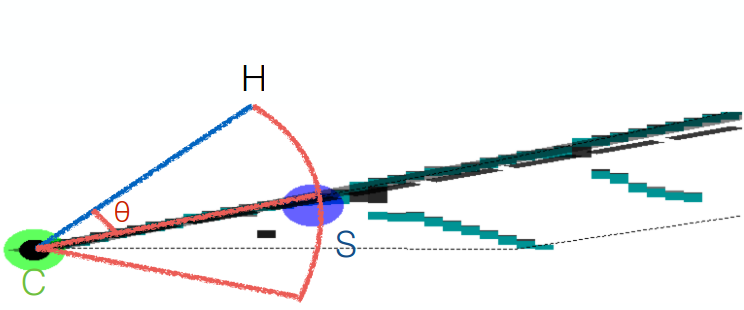
\includegraphics[width=0.7\textwidth]{figures/dQdx_hitselection.png}
\caption{Image showing a detail of the beginning of a shower cluster, highlighting the reconstructed start-point (green circle), showering-point (blue circle), the cluster opening angle $\theta$, and the region from which hits will be selected to calculate a dQ/dx quantity.}
\label{fig:dQdx_hitselection}
\end{figure}
\paragraph{}Once the hits in a cluster have been selected, their charge, in ADCs, is first convertex to electric charge, using the calorimetry service, and divided by the wire-pitch calculated accouting for the 3D direction of the shower. The median value of the dQ/dx calculated for all selected hits is then taken as a measure of the dE/dx of the shower.
\paragraph{}This operation is performed on all planes for which a cluster associated to the input shower is present.

\subsection{dEdxFromdQdx}
\paragraph{}This algorithm simply takes the reconstucted dQ/dx calculated on all planes for which an associated cluster is present, and uses the Modified Box Model for ion recombination to calculate a dE/dx value in MeV/cm.


\subsection{LinearEnergy}
\paragraph{}This algorithm reconstruct the shower energy based on the 2D hits associated with the shower. For each plane on which a cluster associated to the shower is present, the charge from all hits in that cluster is integrated. The hit charge in ADCs is converted to electric charge using the LArLite calorimetry service. At this stage two corrections are applied before reconstructing an energy value in MeV:
\begin{itemize}
\item \textbf{Lifetime correction} : the charge of each hit is mutliplied by a correction factor computed as the exponential of the total drift time for that hit, over the electron lifetime. The hit drift time is calculated using the hit x-position, which was calculated assuming T0 of the hit is the same as the trigger time. The electron lifetime is fetched from the \texttt{larutil::DetectorProperties} service. This value is currently fixed at 8 ms.
\item \textbf{Recombination Correction} : a constant recombination correction is applied to all hits. The recombination factor is calculated assuming all hits in the shower are MIP-like. Currently, the recombination factor is calculated using the Modified Box Model described by ArgoNeuT {\color{red} [reference]} and as parametrized in LArSoft, using an electric field of 237 V/cm. A fixed assumed dE/dx value of 2.3 MeV/cm is used to extract a recombination value of 0.66.
\end{itemize}
After a lifetime and recombination correction has been applied, the summed cluster charge in MeV is taken as the measure of the shower energy for each plane on which an associated cluster is present. Finally, an overall shower energy is calculated. This is done by taking the reconstructed energy on the collection-plane, if a cluster on this plane is associated with the shower, or by averaging the reconstructed energy on the two induction planes.
